\chapter{Specyfikacja wymagań}
W tym rozdziale zawarto wymagania postawione programowi przeznaczonemu do odczytywania notacji muzycznej z plików graficznych oraz konwersją odczytanych danych do formatu MIDI.

\section{Wymagania biznesowe}
Nazwa programu to "Photo-2-MIDI". Przeznaczeniem oprogramowania jest umożliwienie użytkownikom zdigitalizowanie w przystępny sposób drukowanych zapisów nutowych ze zdjęć lub skanów do plików MIDI.

\section{Słownik skrótów i pojęć}

	\begin{enumerate}
		\item Notacja muzyczna, pismo nutowe, zapis nutowy - symboliczny język reprezentujący odbieraną słuchowo muzykę graną na instrumentach, czy też śpiewaną przez ludzki głos, przy pomocy symboli reprezentujących dźwięki, ich długość oraz wysokość, jak i brak tych dźwięków używając znaków pauz. Przy pomocy takiego języka można zapisać niemal wszystkie cechy dźwięków, takie jak rytmika, melodia, harmonia, dynamika czy artykulacja. W tej pracy pojęcia te będą odnosić się do nowożytnej zachodniej notacji muzycznej.
		
		\begin{figure}
			\centering
			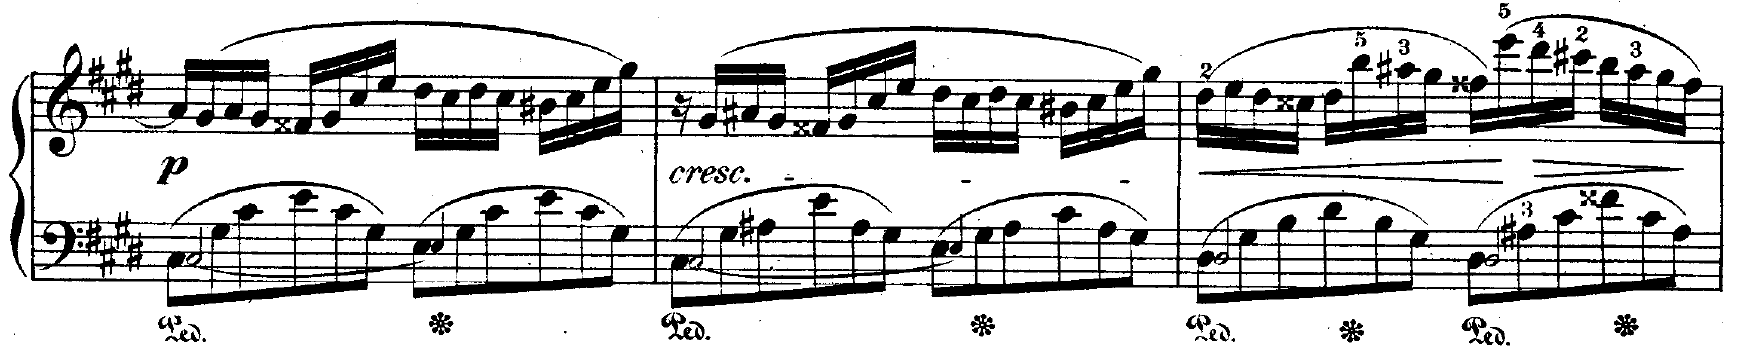
\includegraphics[width=14cm]{images/chopin_fastasie_impromtu_no_4_op_66.png}
			\caption{Fragment \textit{Fantasie-Impromptu cis-moll op. 66} Fryderyka Chopina zapisany w nowożytnej zachodniej notacji muzycznej. }
			\label{fig:chopin_impromptu}
		\end{figure}
		
		\item format MIDI - (ang. Musical Instrument Digital Interface) popularny format plików, który w przeciwieństwie do standardowych formatów audio nie przenosi bezpośrednich informacji o dźwięku, tylko informacje o granych nutach, ich synchronizacji, trwaniu oraz głośności. 
	\end{enumerate}

\section{Wymagania funkcjonalne}
	\begin{enumerate}
		\item Użytkownik może wprowadzić plik lub pliki zawierające drukowane pismo nutowe w standardowej zachodniej notacji nutowej w formatach PNG, JPG, PDF.
	\end{enumerate}
	
	
\section{Wymagania niefunkcjonalne}
Program wymaga do działania:
	\begin{enumerate}
		\item Języka Python w wersji 3.11
		\item Systemu operacyjnego Linux
		\item Około 2 GB wolnej pamięci operacyjnej
	\end{enumerate}